\chapter{Image Compression}

A data compression algorithm transforms the data to occupy a less space. The original data is encoded by a program called encoder, to a compressed representation using a fewer number of bits. Decoder is responsible for decompressing the compressed representation. The compression technique where the decompressed data is exactly same as original data is called as lossless compression otherwise it is known as lossy compression technique because some information is lost during coding-encoding phase.

\begin{figure}[!ht]
    \centering
    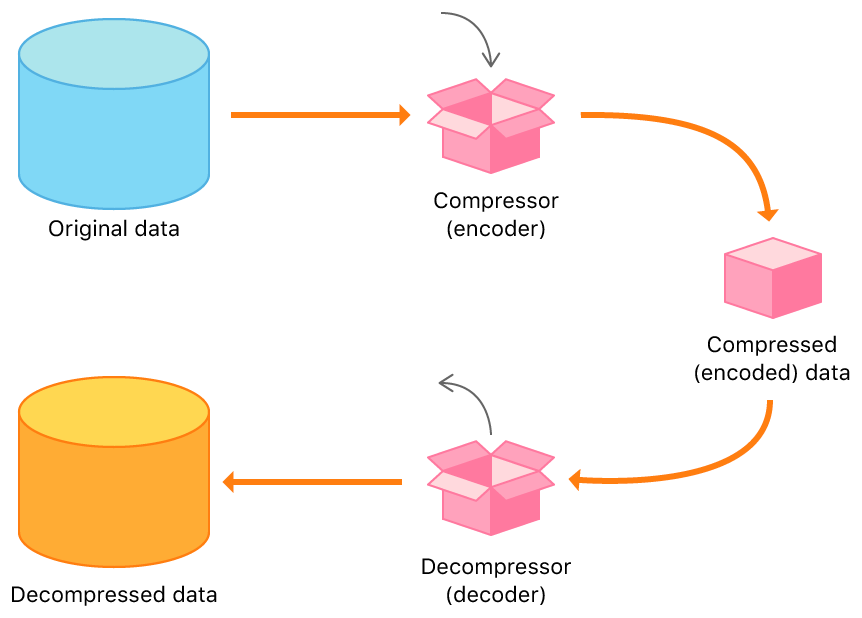
\includegraphics[width=0.50\textwidth]{fig/1-3.png}
    \captionsource{Compression phases}
    {\url{https://developer.apple.com/documentation/compression}}
    \label{fig:phasesCompression}
\end{figure}

Two well-known codecs for image compression are JPEG and PNG. PNG is lossless and JPEG is lossy.

Image compression is very crucial in order to reduce the size of disk space used as well as reduce the amount of internet bandwidth used while loading images. It’s also important to compress images for people accessing the internet via low bandwidth connections.

\section{Section name}

write ....

\section{Conclusion}

This chapter provided details of the some of the existing
distributed algorithms for constructing a CDS in wireless ad-hoc
networks. The results of these evaluations are summarized in table
cut from here. In next chapter, we discuss our distributed
Algorithm I, for constructing a small backbone in ad-hoc wireless
network.


% \ref{table1}
